\documentclass[a4paper]{article}
\usepackage[utf8]{inputenc} 	% codificacao de caracteres
\usepackage[T1]{fontenc}    	% codificacao de fontes
\usepackage[portuges]{babel}  	% idioma
\usepackage[table]{xcolor}    	% linhas coloridas alternadamente
\usepackage{graphicx}
\usepackage{multirow}
\usepackage{soulutf8}			% cor de fundo do texto que aceita utf8
\usepackage{makecell}			% mais de uma linha na célula da tabela
\usepackage[pdftex]{hyperref}
\usepackage[font=small,labelfont=bf]{caption} 



% espaçamento paragrafos
\setlength{\parindent}{0em}
%\setlength{\parskip}{2em}
%\renewcommand{\baselinestretch}{1}

%opening
\title{Universidade do Minho}
\author{Grupo 1}
\date{}

\begin{document}



\begin{center}
	
\includegraphics[scale=0.5]{images/um}
\end{center}


\begin{center}
	\vspace{14ex}
	\LARGE
	Departamento de Informática\\	
	\Huge
	Comunicações por Computador\\
	\vspace{7ex}
	\textbf{{
			\LARGE Trabalho Prático nº 1
	}}\\
	\vspace{5ex}
	{\large 
		Protocolos da Camada de Transporte\\
		Ano Letivo 2020/2021
	}
	\vspace{6ex}
\end{center}



\textbf{Grupo 1 - PL1}\\

Ana Filipa Pereira		A89589\\
Carolina Santejo		A89500  \\
Raquel Costa			A89464 \\




\newpage

\tableofcontents

\newpage


\section{Questões e Respostas}

	\subsection{ Questão 1} 
\textbf{P: Inclua no relatório uma tabela em que identifique, para cada comando executado, qual o protocolo de aplicação, o protocolo de transporte, porta de atendimento e overheadde transporte, como ilustrado no exemplo seguinte:\\}

R:
\begin{table}[h!] %Inserir tabela
\begin{center}
\begin{tabular}{|m{7em}|m{7.5em}|m{7.5em}|m{7.5em}|m{7.5em}|}
\hline
Comando usado (aplicação)    &Protocolo de Aplicação (se aplicável) &Protocolo de Transporte (se aplicável) &Porta de atendimento (se aplicável) & \textit{Overhead} de transporte em bytes (se aplicável)\\
\hline
Ping&  -   &  -  &  -  &  -\\
\hline
traceroute & DNS Protocol   &  UDP  &  33453   &  8   \\
\hline
telnet& telnet & TCP & 57548& 20 \\
\hline
ftp& ftp & TCP & 21 & 20 \\
\hline
Tftp& tftp & UDP & 69 & 8  \\
\hline
browser/http& http & TCP & 34282& 20  \\
\hline
nslookup& DNS & UDP & 53 &  8\\
\hline
ssh& ssh & TCP & 54766 &  20\\
\hline

\end{tabular}
\end{center}
\end{table}


\begin{center}
	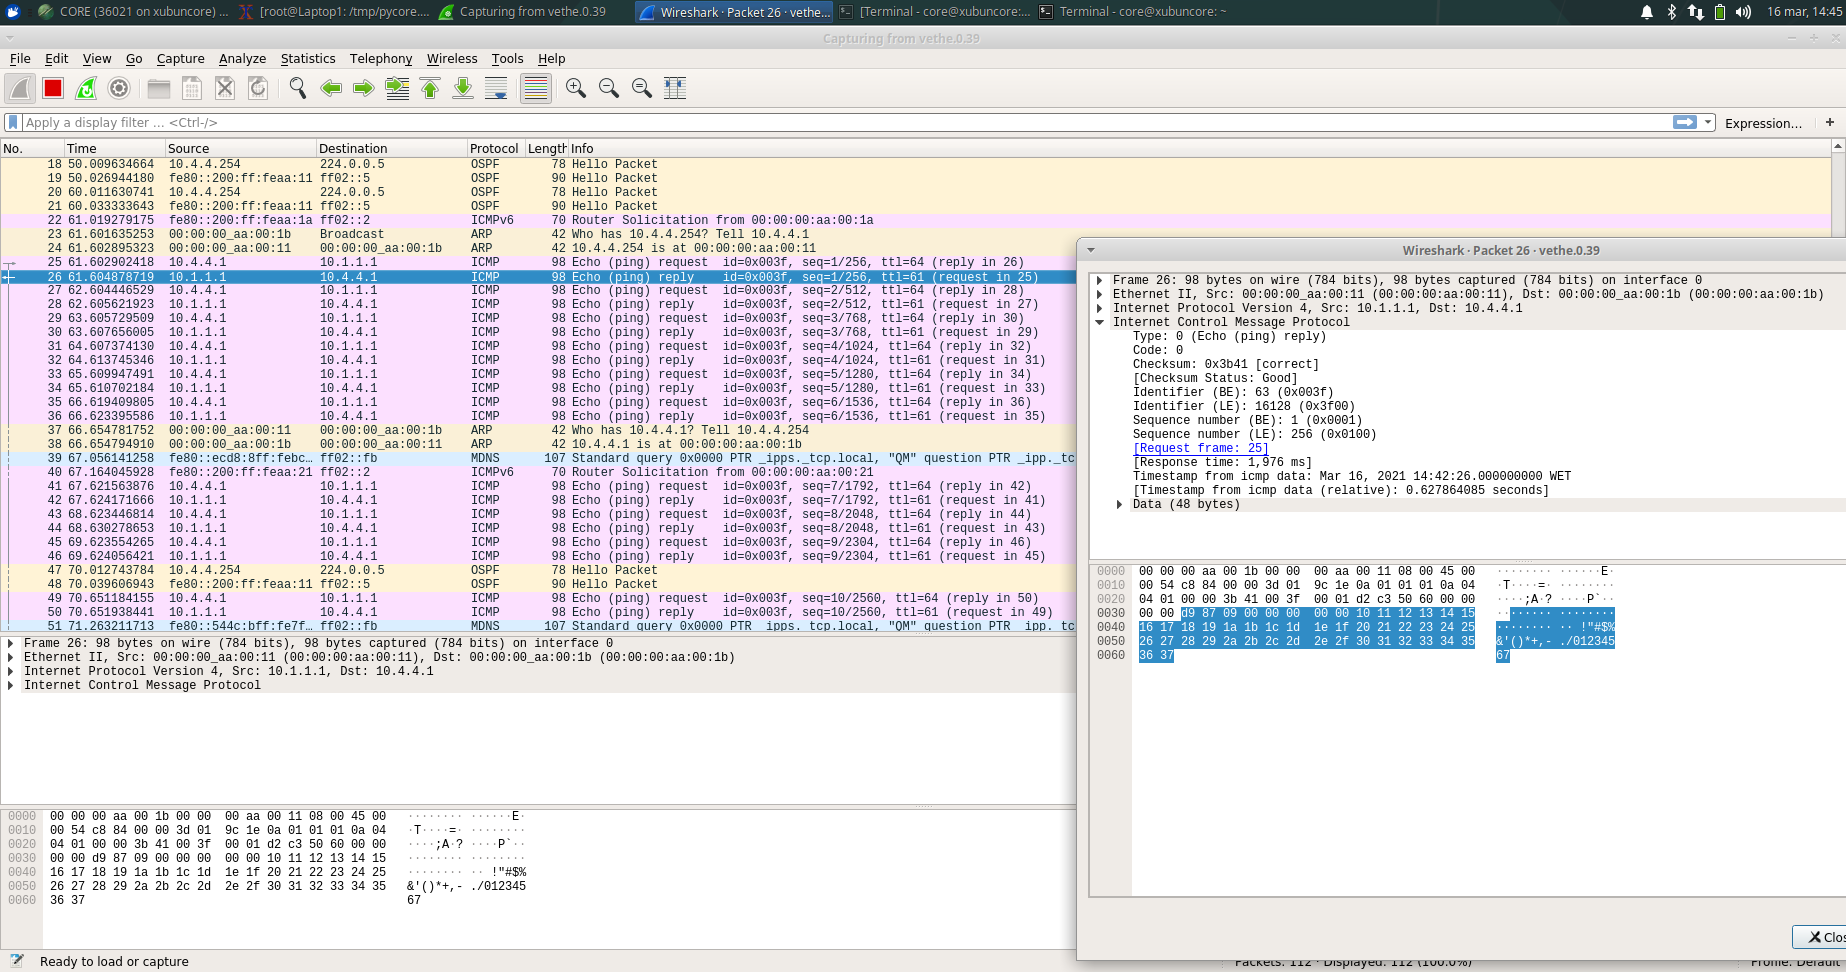
\includegraphics[scale=0.23]{images/ping}
	\captionof{figure}{Ping.}
\end{center}

\begin{center}
	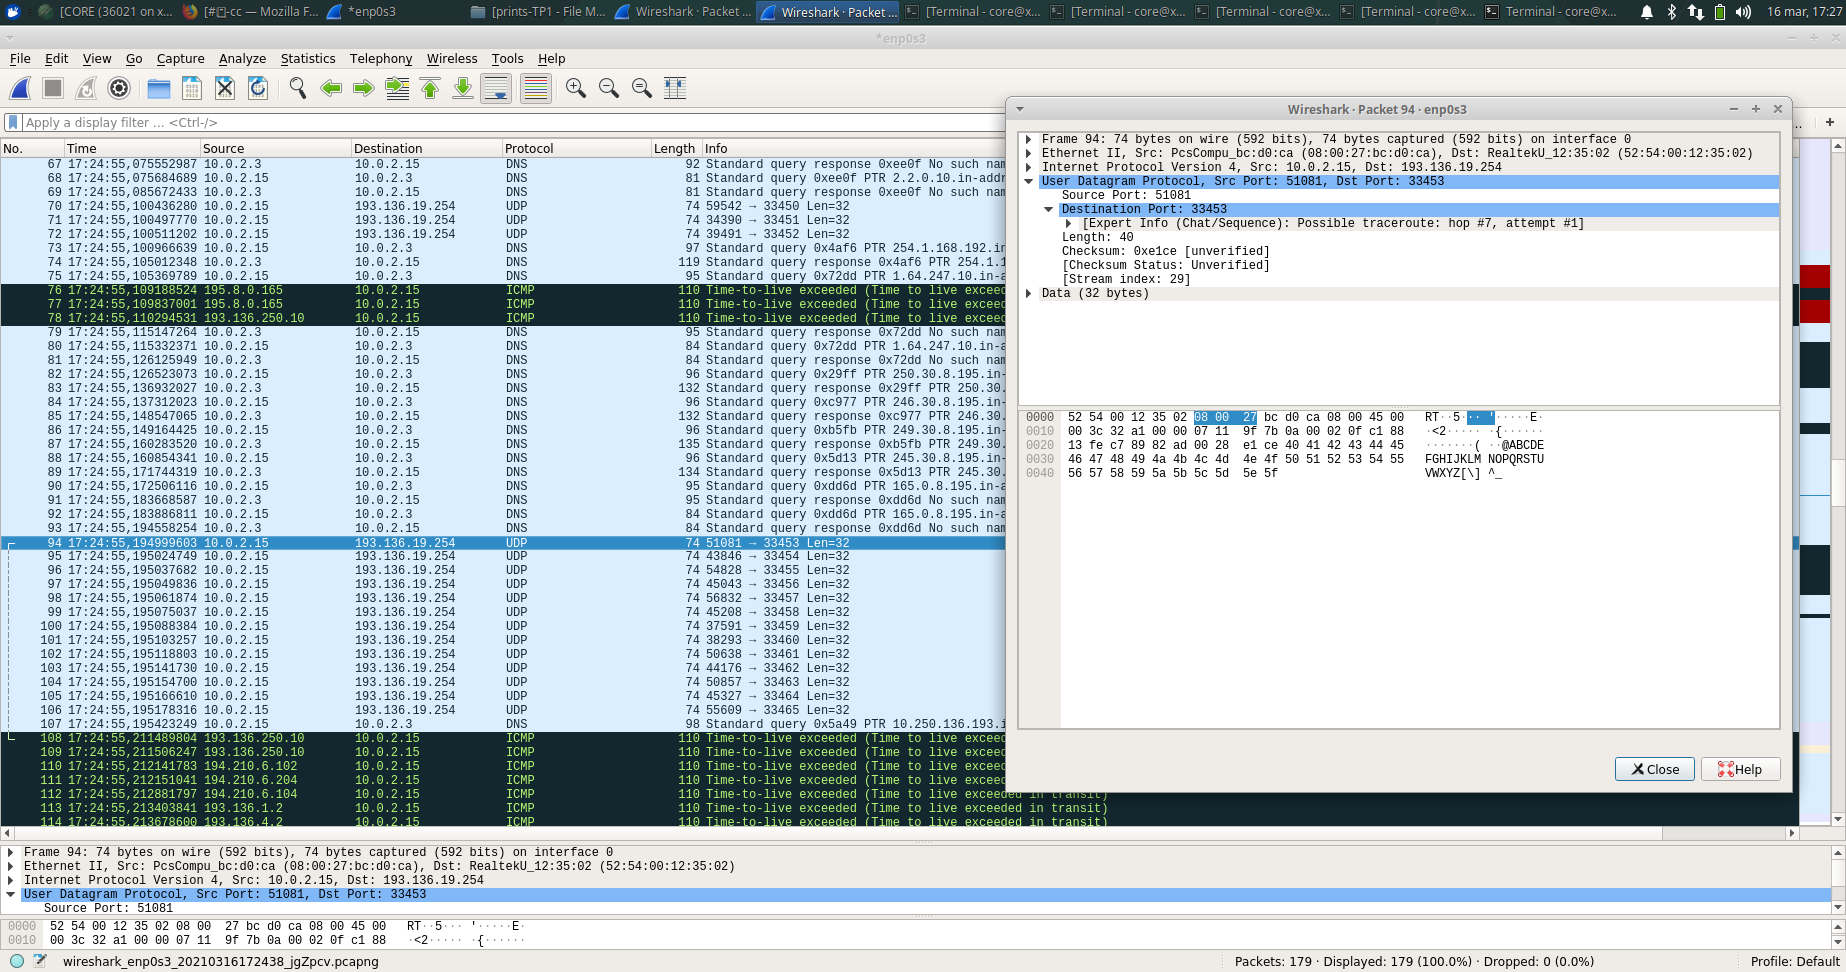
\includegraphics[scale=0.23]{images/traceroute}
	\captionof{figure}{Traceroute.}

\end{center}

\begin{center}
	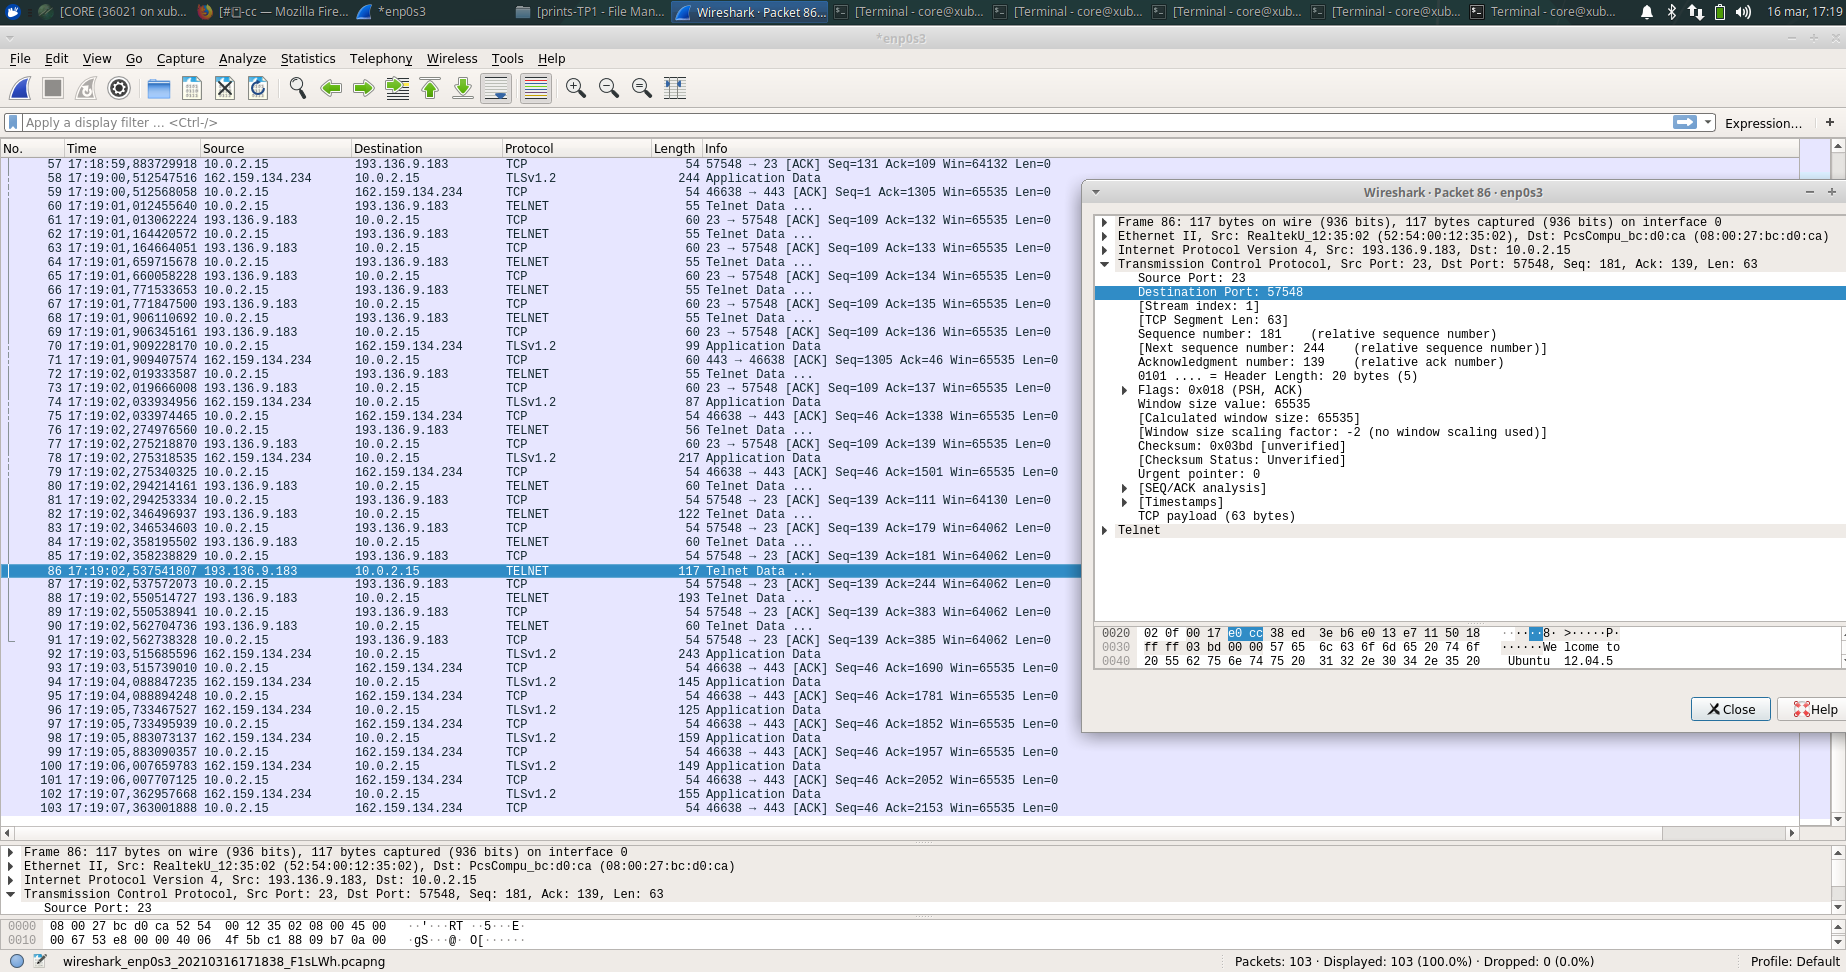
\includegraphics[scale=0.23]{images/telnet}
	\captionof{figure}{Telnet.}
\end{center}

\begin{center}
	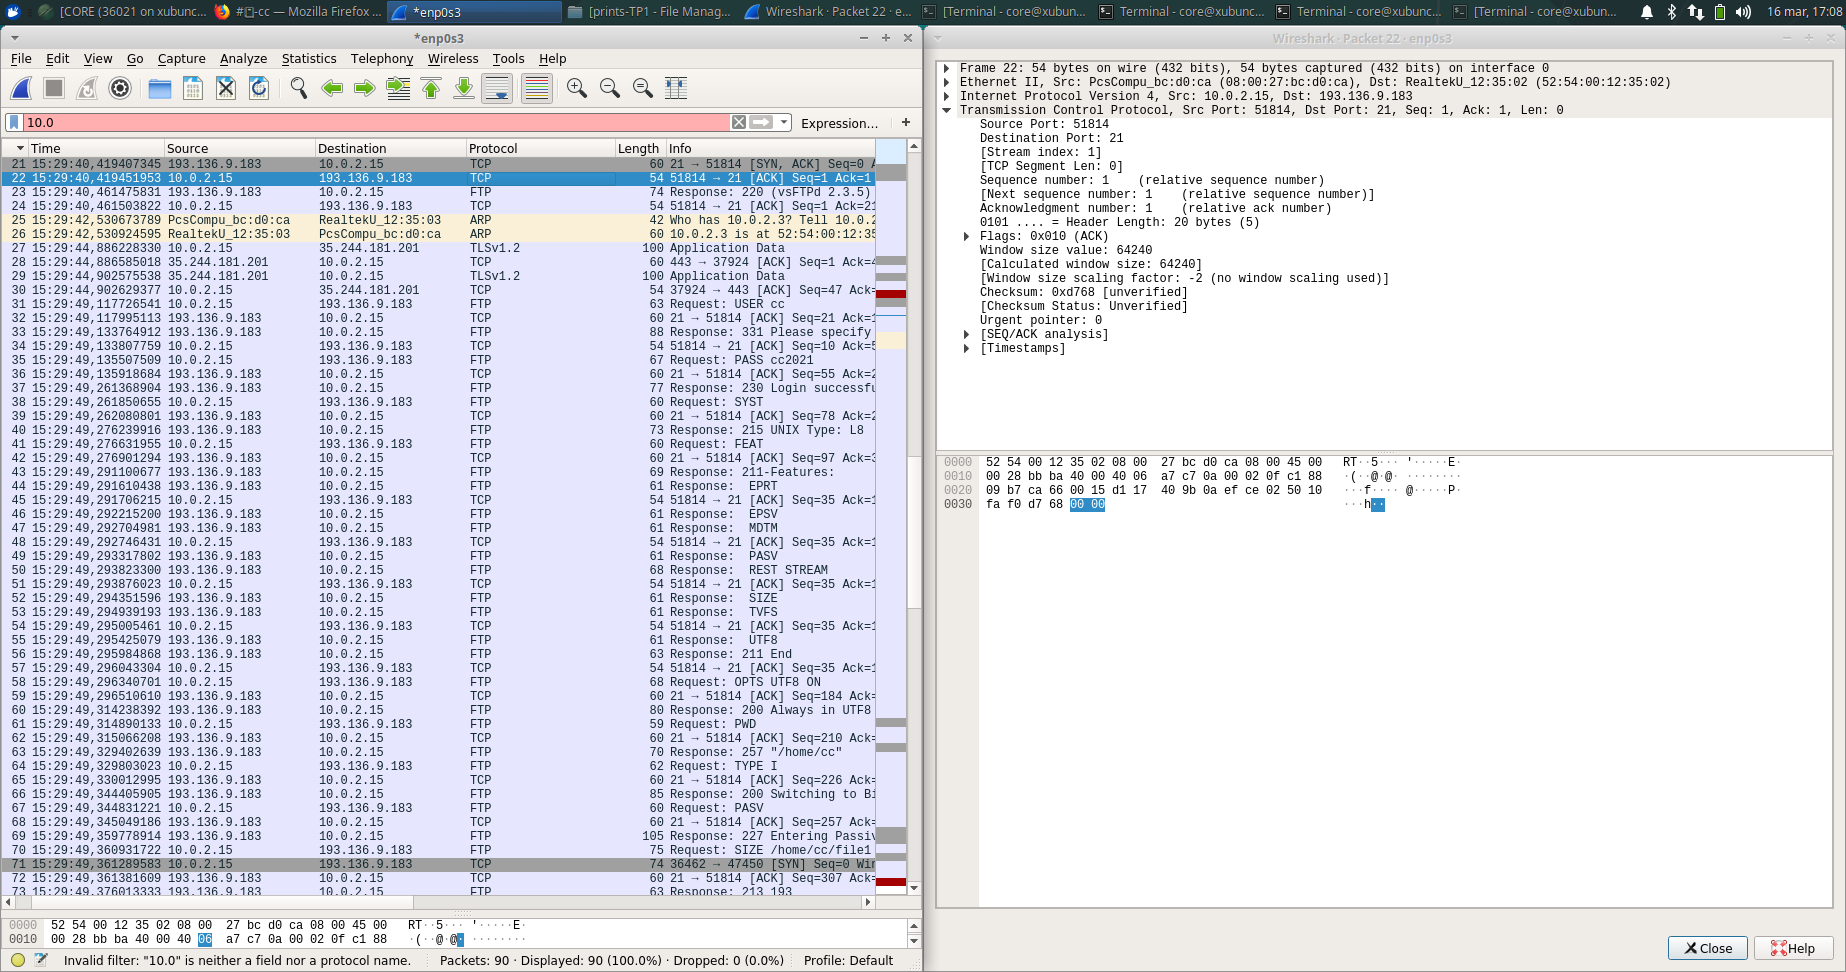
\includegraphics[scale=0.23]{images/FTP}
	\captionof{figure}{Ftp.}
\end{center}

\begin{center}
	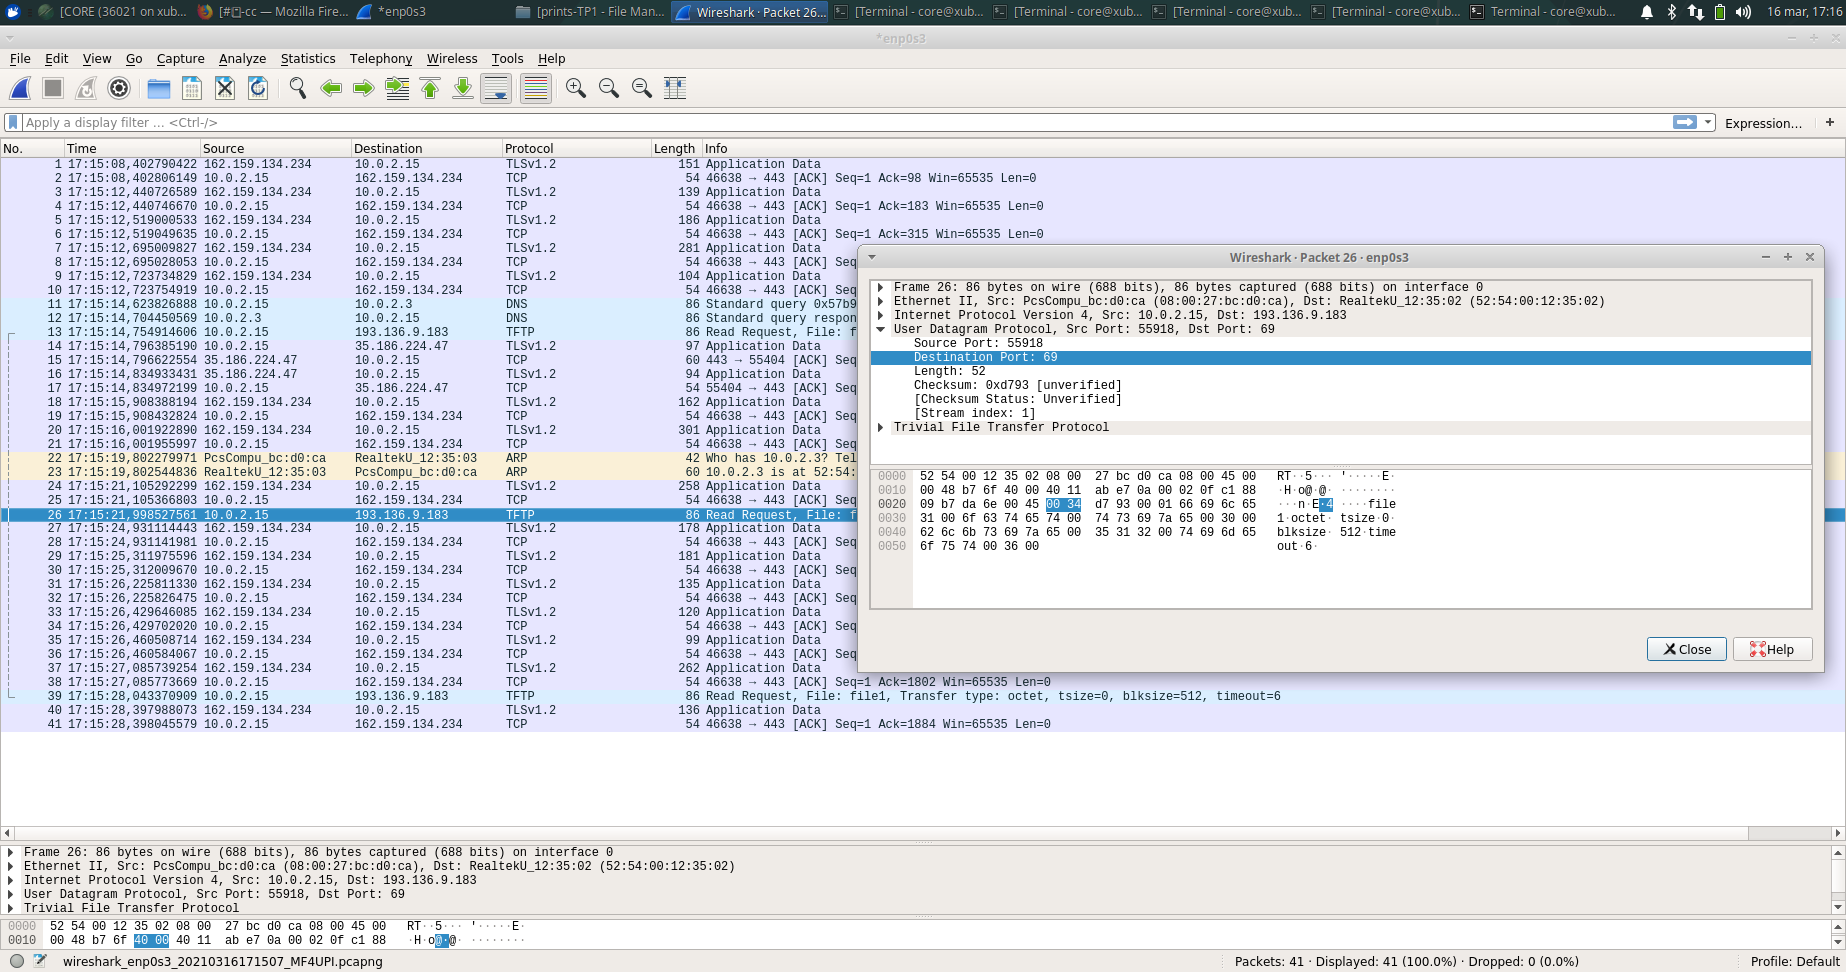
\includegraphics[scale=0.23]{images/tftp}
	\captionof{figure}{Tftp.}
\end{center}

\begin{center}
	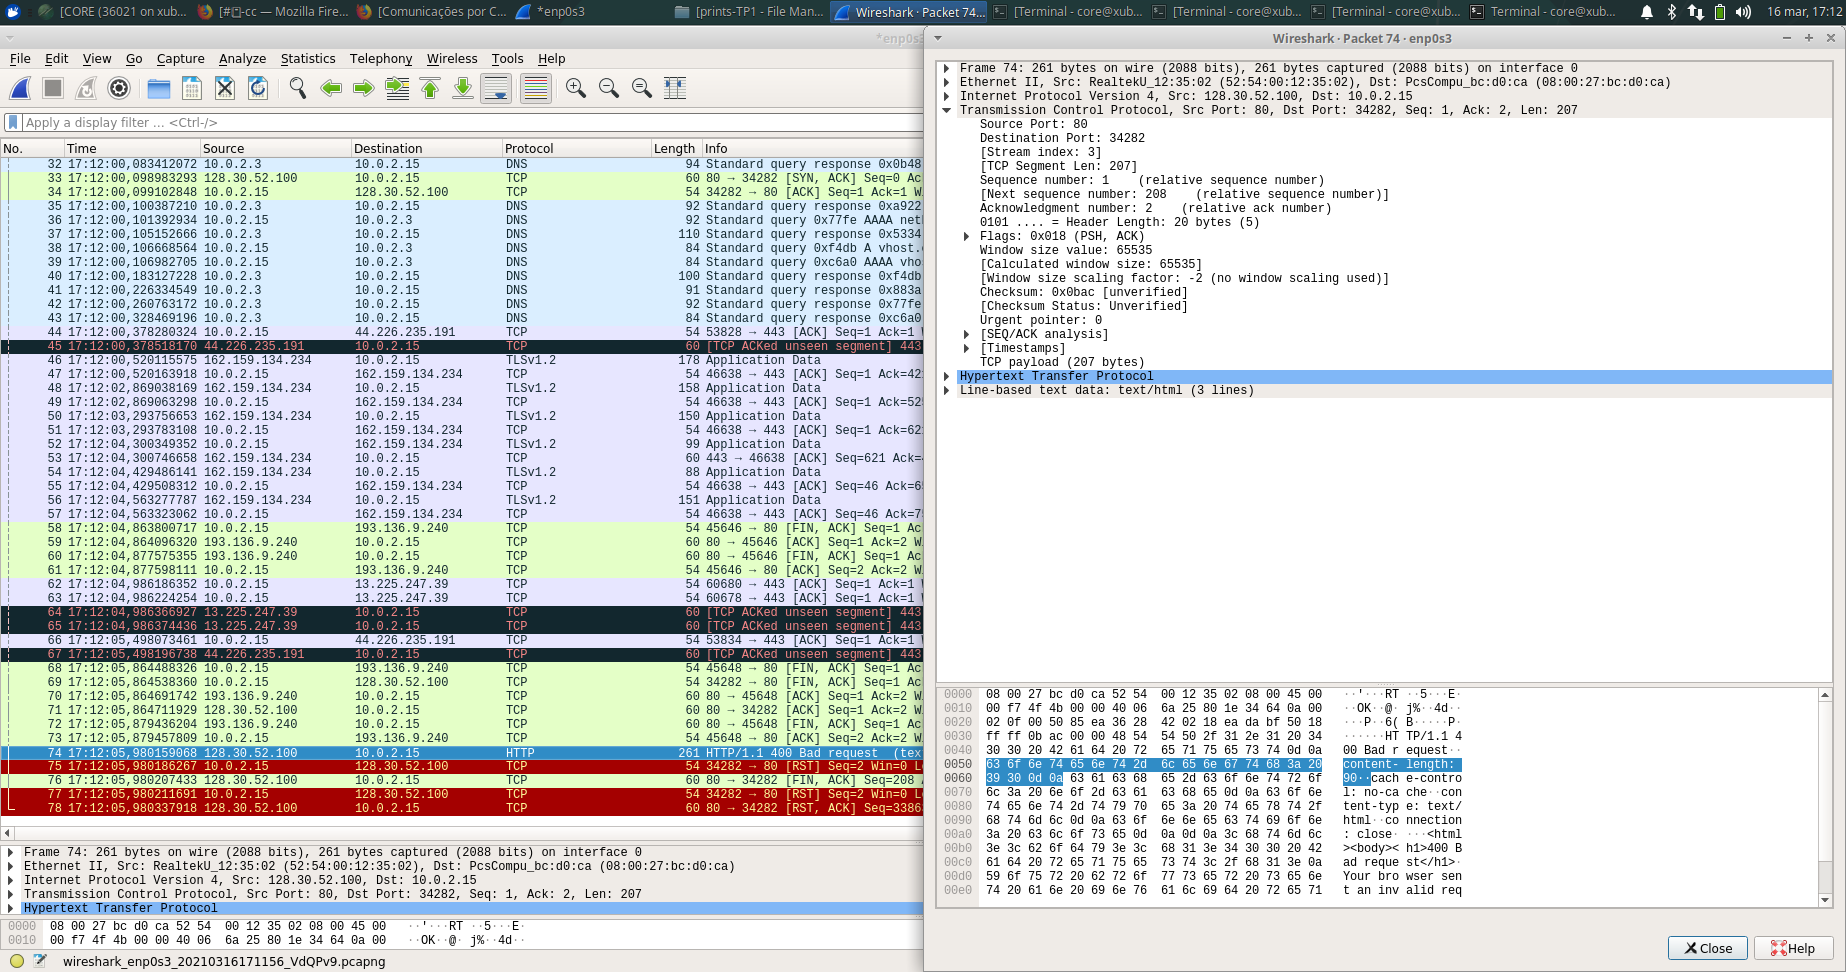
\includegraphics[scale=0.23]{images/http}
	\captionof{figure}{Browser/http.}
\end{center}

\begin{center}
	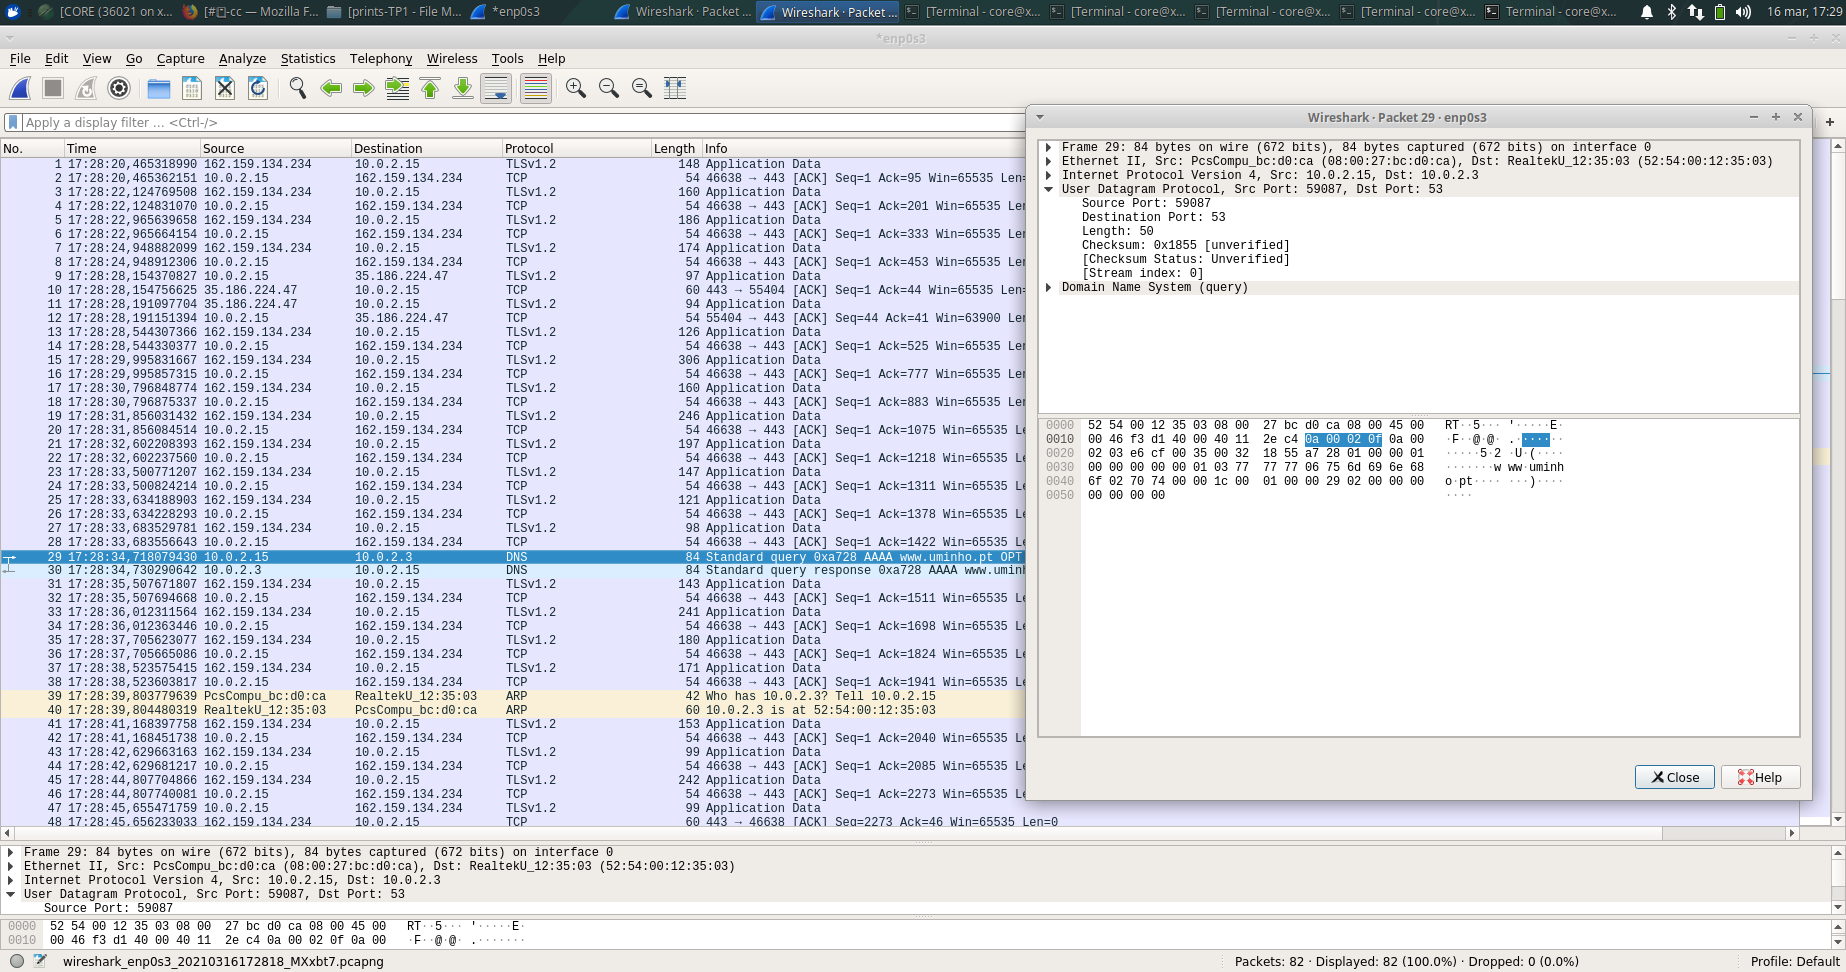
\includegraphics[scale=0.23]{images/nslookup}
	\captionof{figure}{Nslookup.}
\end{center}

\begin{center}
	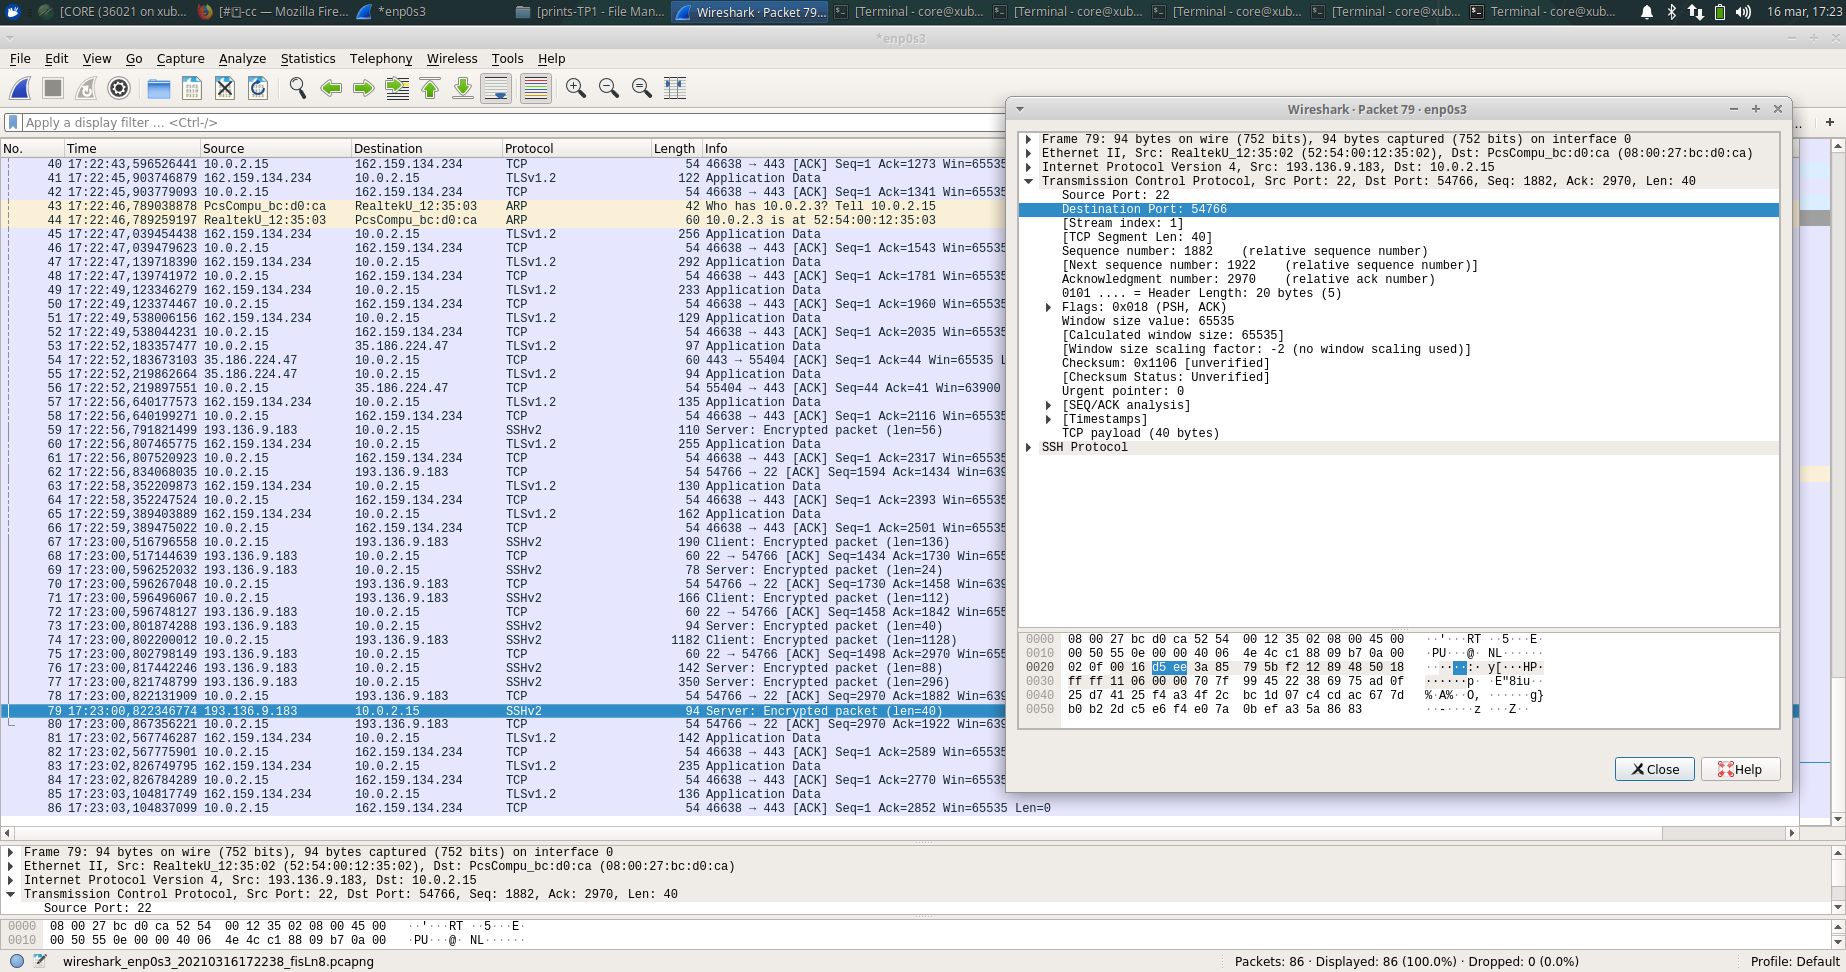
\includegraphics[scale=0.23]{images/ssh}
	\captionof{figure}{Ssh.}
\end{center}


\newpage

	\subsection{ Questão 2}
\textbf {P: Uma representação num diagrama temporal das transferências da file1por FTPe TFTPrespetivamente. Se for caso disso, identifiqueas fases de estabelecimento de conexão, transferência de dados e fim de conexão. Identifica também claramente os tipos de segmentos trocados e os números de sequência usados quer nos dados como nas confirmações. (Nota:a transferência por FTP envolvemais que uma conexão FTP, nomeadamente uma de controlo [ftp] e outra de dados [ftp-data]. Faça o diagrama apenas para a conexão de transferência de dados do ficheiro mais pequeno)\\}

R:

\begin{center}
	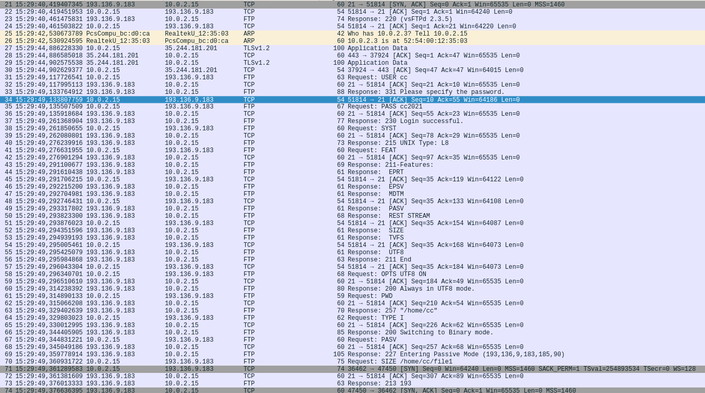
\includegraphics[scale=0.6]{images/ftp1.1}
	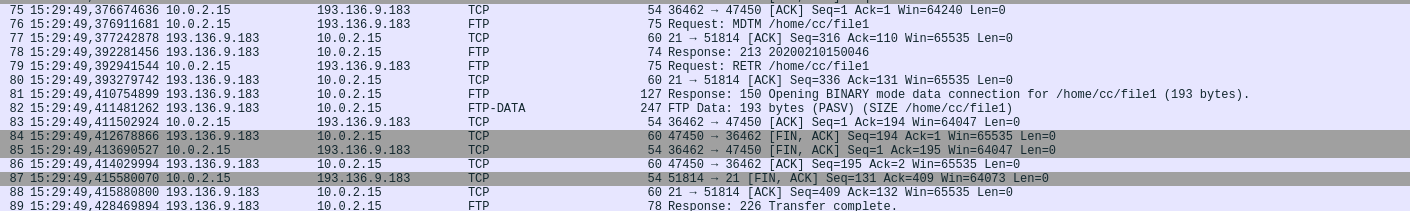
\includegraphics[scale=0.3]{images/ftp1.2}
	\captionof{figure}{Ftp - Captura de tráfego.}
\end{center}

\begin{center}
	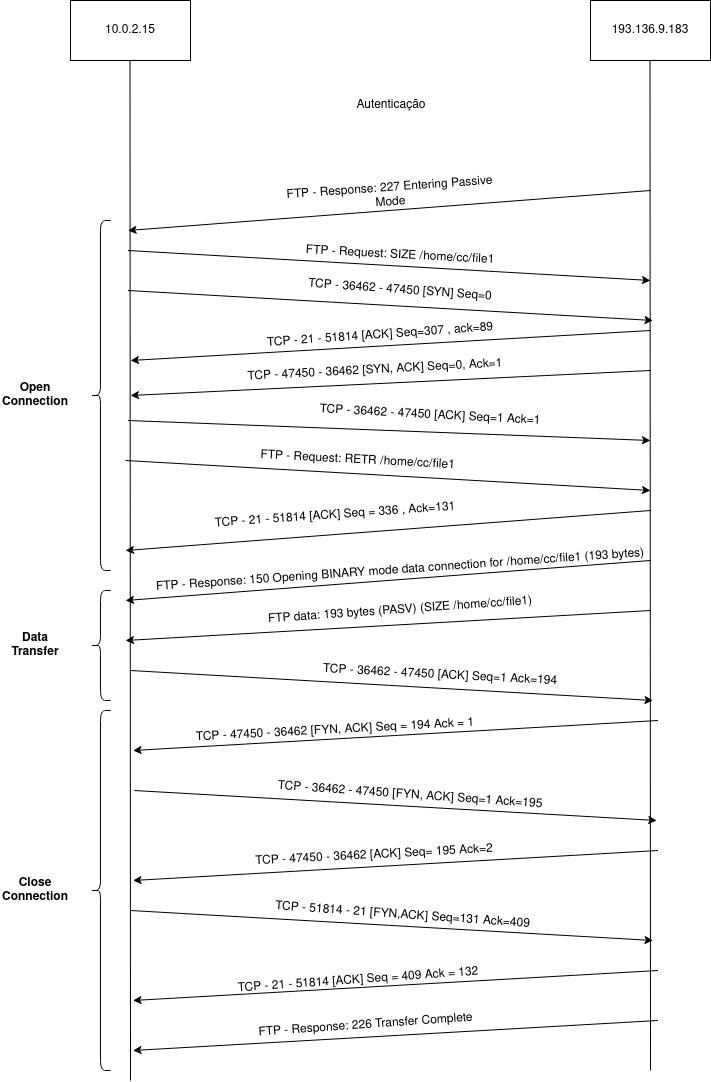
\includegraphics[scale=0.5]{images/diagramaFTP}
	\captionof{figure}{Ftp - Diagrama Temporal}
\end{center}

\newpage
\textbf{NOTA:} Não foi possível voltar a capturar o tráfego do acesso em tftp para cc2021.ddns.net, como forma de justificação do diagrama temporal representado na Figura 11. Para tal, pedimos que se tenha em conta a Figura 5.

\vspace{8ex}

\begin{center}
	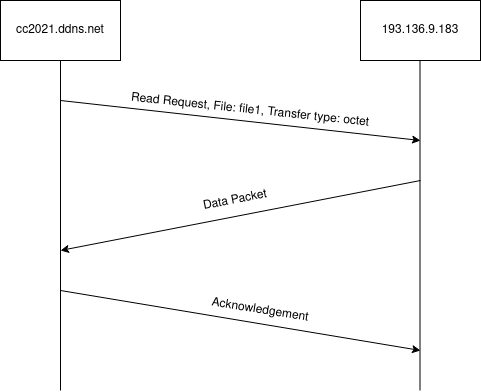
\includegraphics[scale=0.5]{images/diagramaTFTP}
	\captionof{figure}{Tftp - Diagrama Temporal}
\end{center}


\vspace{8ex}

	\subsection{ Questão 3}
\textbf{P: Com base nas experiências realizadas, distinga e compare sucintamente as quatro aplicações de transferência de ficheiros que usou nos seguintes pontos (i) uso da camada de transporte; (ii) eficiência na transferência; (iii) complexidade; (iv) segurança;\\}


R: Pela análise de pacotes no wireshark, podemos comparar as quatro aplicações de transferências de ficheiros em diversos pontos, dos quais destacaremos alguns.
A nível do uso da camada de transporte, as aplicações SFTP, FTP e HTTP utilizam o protocolo TCP, enquanto que a aplicação TFTP utiliza o protocolo UDP.
Quanto á eficiência de transferência podemos afirmar que: a aplicação SFTP utiliza ligações SSH que causam maior overhead e por isso diminuem a eficiência de transmissão. O facto de o SFTP ser fiável, também contribui para esta baixa eficiência. A aplicação FTP tem um elevado overhead e por isso também possui uma baixa eficiência de transferência. A aplicação TFTP tem uma elevada eficiência de transmissão devido ao baixo overhead. A aplicação HTTP possui também uma elevada eficiência de transmissão.
Quanto á complexidade podemos afirmar que: as aplicações SFTP e FTP disponibilizam diversas funcionalidades tornando-os mais complexos. A aplicação TFTP é pouco complexa uma vez que implementa o protocolo UDP, não tendo este, muitas funcionalidades (por exemplo, não tem mecanismos de autenticação). A aplicação HTTP é pouco complexa.
Por fim, quanto á segurança podemos afirmar que: a aplicação SFTP é considerada segura na medida em que recorre a autenticação e encriptação de informação. Além disto, a utilização de ligações SSH a tornam também mais segura. A aplicação FTP apesar de recorrer á autenticação, é pouco segura. Por exemplo, durante a análise de pacotes utilizando o wireshark, era possível ler as passwords, não havendo qualquer tipo de encriptação. A aplicação TFTP não recorre a autenticação ou encriptação, sendo por isso pouco seguro. A aplicação HTTP recorre a autenticação, mas não recorre á encriptação, sendo por isso, pouco seguro.

\vspace{12ex}

	\subsection{ Questão 4}   
\textbf {P: As  características  das ligações  de  rede  têm  uma  enorme  influência  nos  níveis  de  Transporte  e  de  Aplicação.  Discuta, relacionando a resposta com as experiências realizadas, as influências das situações de perda ou duplicação de pacotes IP no desempenho global de Aplicações fiáveis (se possível, relacionando com alguns dos mecanismos de transporte envolvidos).\\}


R: Observando a figura x podemos verificar que houve perda de 5\% dos pacotes enviados e 3 foram duplicados, isto porque havia problemas de rede e não havia nenhum protocolo para garantir o transporte ponto a ponto.
Por outro lado, na figura y podemos comprovar pela captura que foi utilizado o protocolo TCP, que garante a entrega de todos os pacotes enviados. No entanto, isto implica o envio de várias mensagens de controlo, aumentando assim a complexidade da transmissão e originando uma maior sobrecarga da rede.
Quanto ao UDP, estamos perante um protocolo muito menos complexo mas não fiável, o que implica ser a camada superior (aplicação) a garantir a receção dos dados. 
Este pode ser implementado em casos que seja necessário enviar pacotes rapidamente.

\begin{center}
	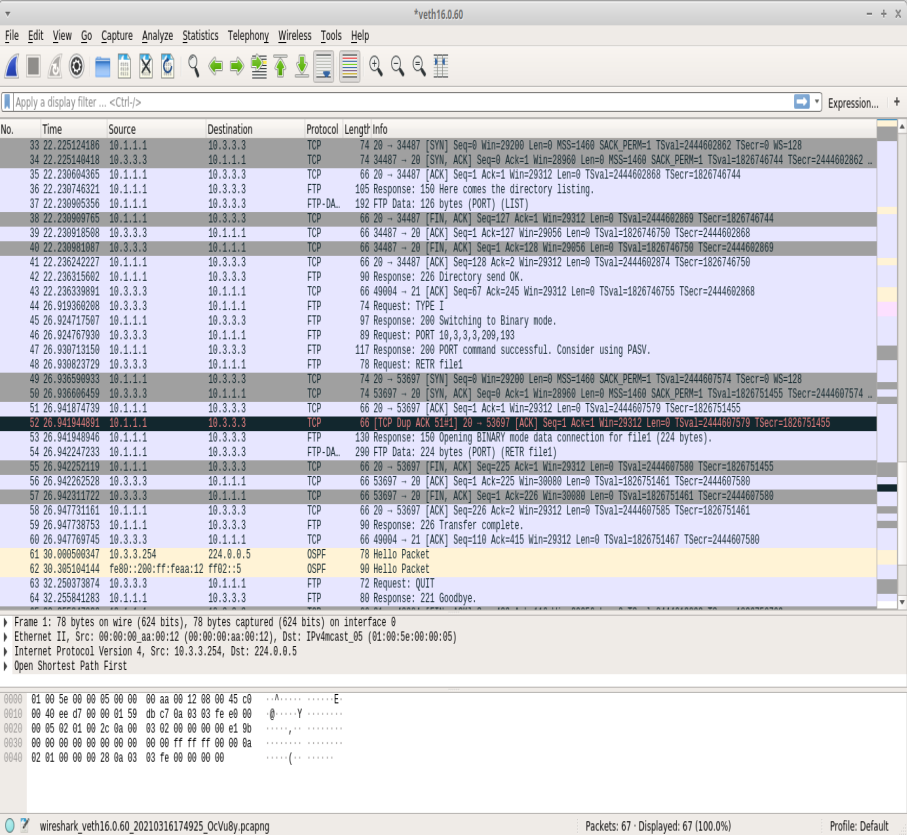
\includegraphics[scale=0.6]{images/4}
	\captionof{figure}{Captura de Tráfego da transferência do ficehiro file1.}
\end{center}

\vspace{8ex}

\begin{center}
	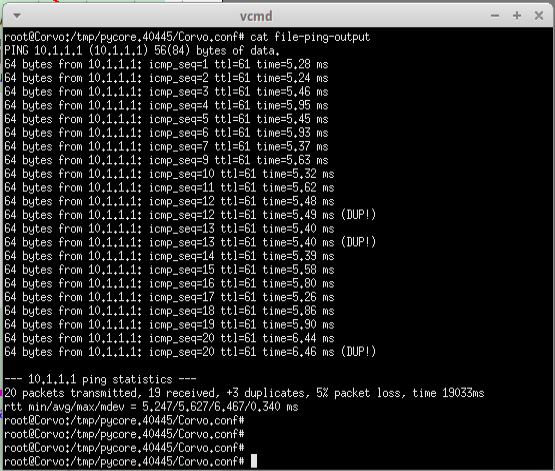
\includegraphics[scale=0.7]{images/4.2}
	\captionof{figure}{Ping do laptop Corvo para o Server1.}
\end{center}

\newpage
\section{Conclusões}

Ao longo deste guião, o grupo conseguiu aplicar e consolidar todos os conceitos abordados durante as aulas teórico-práticas, nomeadamente, a camada de transporte e os diversos protocolos de transporte e aplicacionais existentes.
A nível de protocolos de transporte, o TCP e o UDP foram os que receberam maior atenção.
Por fim, foi feita, utilizando a ferramenta wireshark, uma análise  do tráfego gerado pelo uso dos vários protocolos.


\end{document}